\section{Results and Discussion}

This section presents the full optical characterisation of a single-photon emitter identified in an hBN nanocrystal, including its purity, brightness, and indistinguishability. Although several emitters were partially characterised, their instability, typically disappearing after a few hours to several weeks, meant only one emitter was studied comprehensively. This instability is likely due to the significant detuning between the 450~nm excitation laser and the ZPL wavelengths (between 600 and 700~nm), with excess energy dissipating as lattice vibrations and inducing local heating and structural changes. Despite this limitation, results from other emitters will be included where relevant for completeness. The fully characterised emitter is denoted with `\textcolor{red}{*}' and referred to as the 710~nm defect.


\subsection{Emitter Characterisation}

\subsubsection{Spectrum and Lifetime \label{spec-lt}}

\begin{figure}[h!]
    \centering
    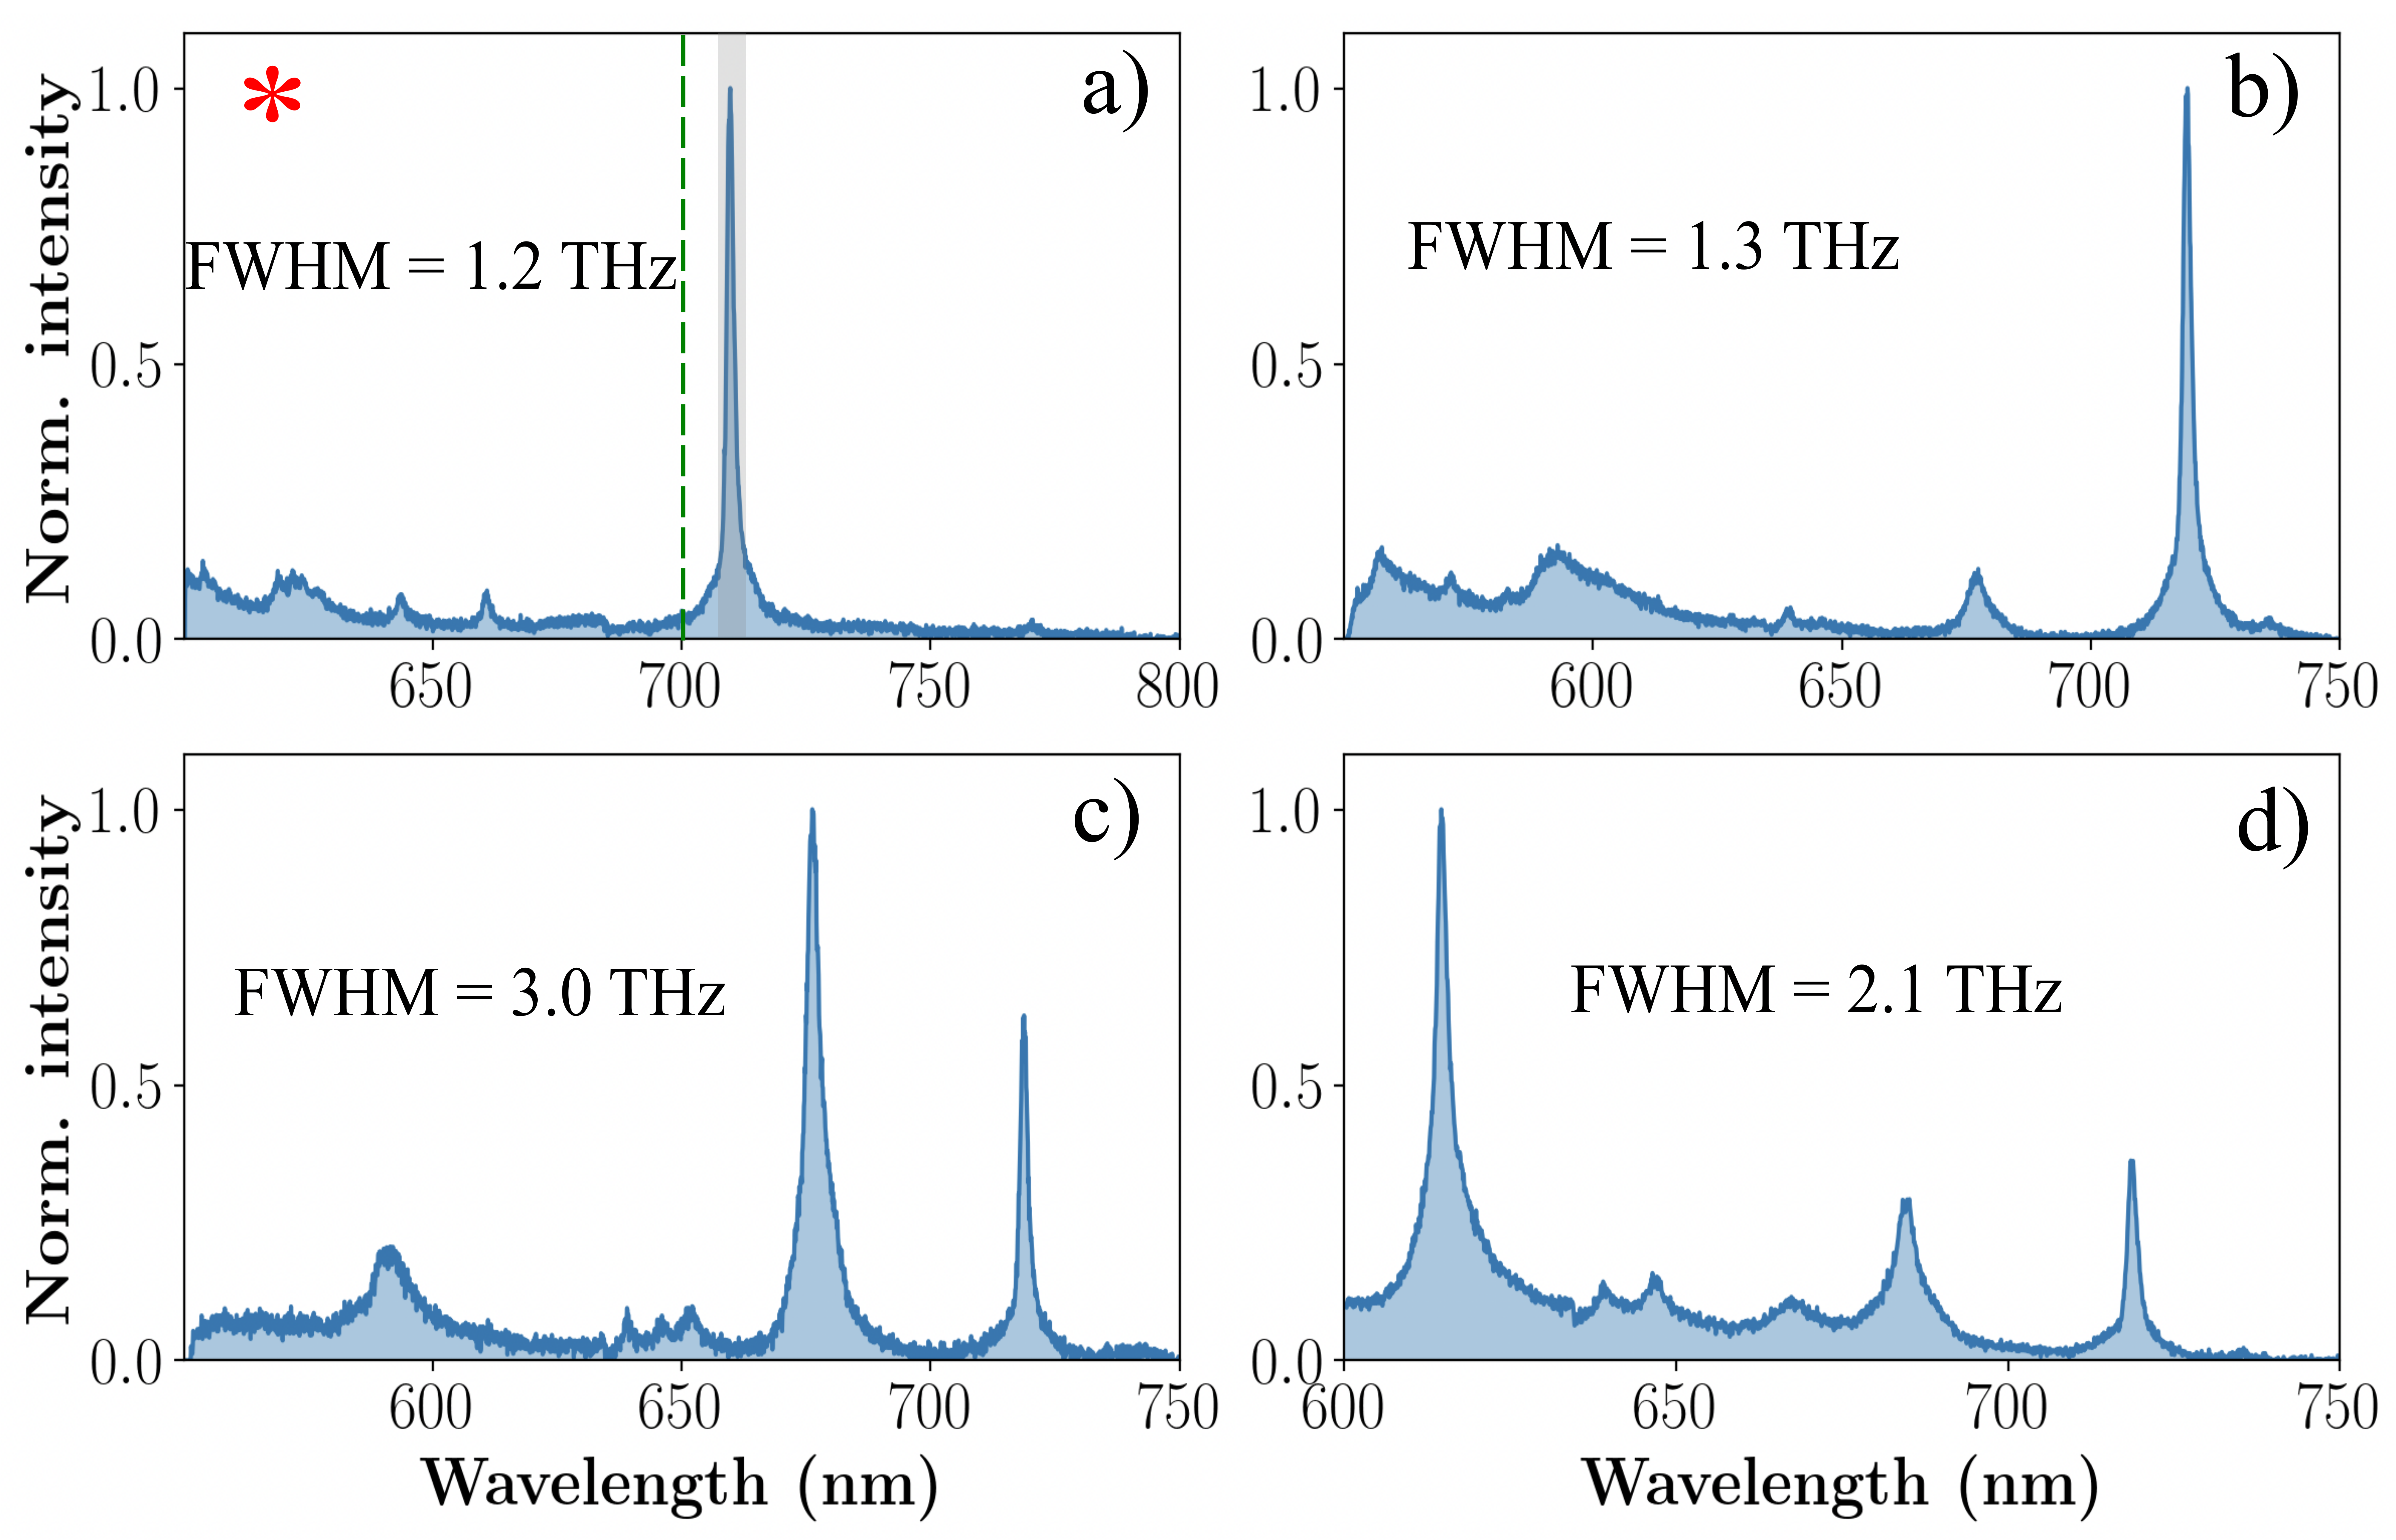
\includegraphics[width=0.85\linewidth]{Figures/Spectrums.png}
    \caption{Various spectra of different hBN defect emitters. The red star indicates the spectrum of the emitter which is fully characterised in this work. a) Normalised spectrum centred at 710 nm with a FWHM of 1.2 THz. The green dashed line and greyed out area indicate different filtering schemes used during measurements b) Normalised spectrum centred at 720 nm with a FWHM of 1.3 THz c) Normalised spectrum centred at 680 nm with a FWHM of 3.0 THz d)
    Normalised spectrum centred at 615 nm with a FWHM of 2.1 THz}
    \label{fig:spectra}
\end{figure}


Fig.~\ref{fig:spectra} shows the background corrected PL spectra of various emitters, with ZPLs centred between 615 nm and 720 nm. Each ZPL is fitted with a Lorentzian function and the FWHM extracted, yielding linewidths between 1.2 THz and 3 THz, with an average of 1.9 THz. Across all emitters, 'shoulder' side features are present at the base of the ZPL. These features correspond to the low energy zone-centre out-of-plane optical mode (ZO$(\Gamma)$) of hBN, which has a frequency of $~110$ cm$^{-1}$ (0.0137 eV), corresponding to a spectral shift of approximately 5 nm at a central wavelength of 700 nm \cite{Cusco2016,Jin2017}. 

The 710 nm defect (\textcolor{red}{*}) features a ZPL centred at 710.1 nm (1.746 eV), with a linewidth $\Gamma/2\pi=$1.2 THz. This emitter has a $DW$ factor of 0.32, which is significantly lower than values reported for hBN defect centres at cryogenic temperatures~\cite{Tran2016}, but comparable to those observed in other high-temperature measurements~\cite{Ari2025}. This is expected as phonon interactions at higher temperatures contribute to a broadened linewidth. The $DW$ factor is calculated by integrating the intensity of the ZPL up to the onset of the side features, see dashed black lines in Fig.~\ref{fig:spectra}a, and dividing it by the integrated intensity at lower energies from the green dashed line, Fig.~\ref{fig:spectra}a. It is worth noting that this $DW$ factor may be slightly overestimated, as a portion of the PSB overlaps with the spectral edge of the DBR mirror stopband, reducing its collection efficiency relative to the ZPL, see appendix. 

\begin{figure}[h]
    \centering
    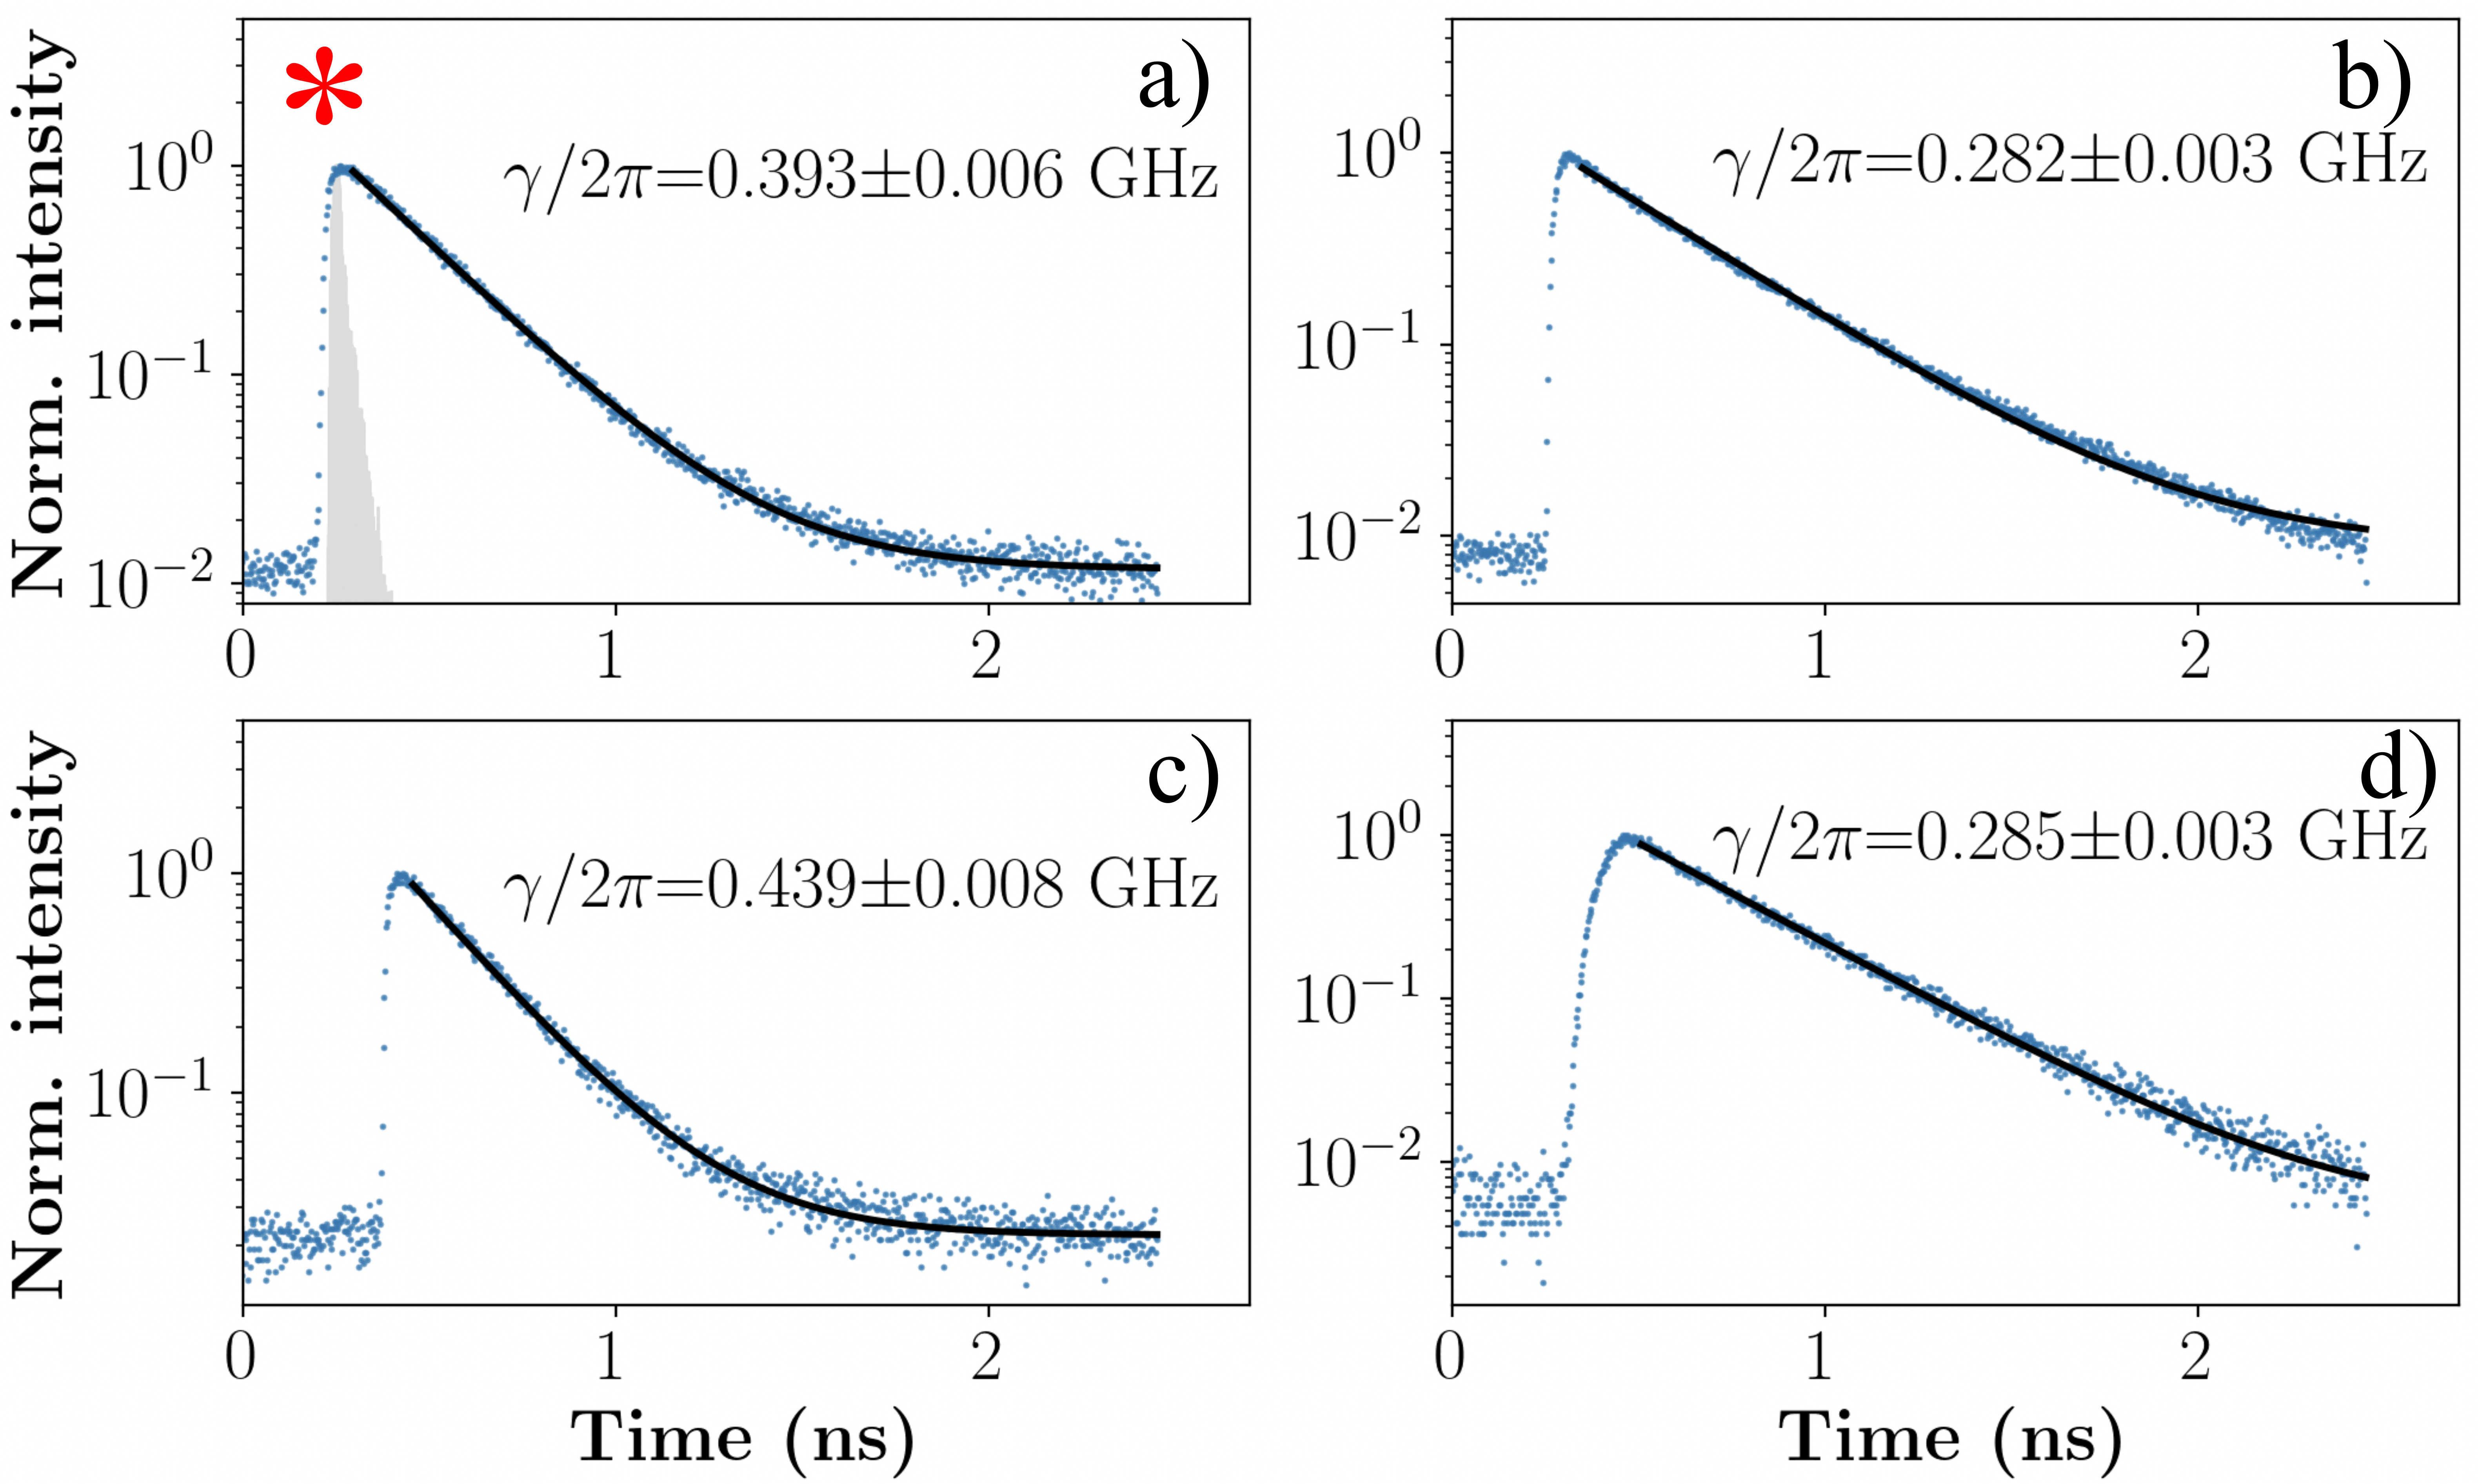
\includegraphics[width=0.9\linewidth]{Figures/Lifetimes.png}
    \caption{Lifetime measurement data (blue dots) and exponential fit (black line) for four different defects. a) The 710 nm defect displays a spontaneous decay rate of 0.393$\pm$0.006 GHz and shows excellent agreement with a signle-exponential fit. The grey area represents the APD's IRF. Similar decay rates are exhibited by other emitters (b,c,d) found on the sample.}
    \label{fig:lifetimes}
\end{figure}

Fig.~\ref{fig:lifetimes} presents the lifetime measurements of four different emitters. The lifetimes vary between 2.27 ns and 3.54 ns, which correspond to Fourier transform-limited decay rates between 0.282 GHz and 0.439 GHz, with an average of 0.350 GHz. The corresponding Fourier transform-limited linewidths are around ten thousand times narrower than the FWHMs shown in Fig.~\ref{fig:spectra}, indicating the presence of strong dephasing mechanisms. The 710 nm defect exhibits a lifetime of $2.54\pm0.04$ ns (0.393$\pm$0.006 GHz). The initial uncertainty in the lifetime measurement was obtained by assuming Poissonian statistic statistics for the photon counts in each time bin, and the error in each bin taken as the square root of the value. This yielded an uncertainty of 0.01 ns. This is smaller than the timing jitter of the APD used for measuring, 40 ps Fig.~\ref{fig:apd-characterisation}. Strictly speaking, the lifetime measurement should be deconvolved with the APD IRF (grey area Fig.~\ref{fig:lifetimes}a). However, it is evident that the IRF is significantly narrower than the spontaneous decay rate, making deconvolution unnecessary. Therefore, an overall timing uncertainty of 0.04 ns was adopted for the measurement.


\subsection{PIB of the 710 nm Defect}

\subsubsection{Brightness}

The brightness of the 710 nm defect can be found by measuring its saturation curve, and extracting the intensity at infinite power. This is invesitgated under both CW and pulsed excitation scheme.

\begin{figure}[h]
    \centering
    
\includegraphics[width=1\linewidth]{Figures/SatCurves.png}
    \caption{Saturation behaviour 710 nm defect under (a) CW excitation and (b) pulsed excitation at a 40~MHz repetition rate. The data is fitted using the standard saturation model, yielding saturation powers of $P_{\text{Sat}}^{\text{cw}} = 0.54 \pm 0.09$~mW and $P_{\text{Sat}}^{\text{p}} = 0.041 \pm 0.003$~mW, respectively.}
    \label{fig:sat-curves}
\end{figure}

Fig.~\ref{fig:sat-curves}a presents the power-dependent emission intensity of the filtered ZPL (grey shaded area Fig.~\ref{fig:spectra}a) under CW excitation. The saturation power at the sample surface extracted from the fit, Eqn.~\ref{eqn:p-sat}, is found to be $P_{\text{Sat}}^{\text{cw}} = 0.54 \pm 0.09$~mW at the sample surface, which corresponds to approximately 8 \% laser power, Fig.~\ref{fig:laser-char}c. The intensity at infinite power under CW excitation is $I_{\infty}^{\text{cw}} = 18.0 \pm 0.4$~kHz, which corresponds to a brightness measured at the detector of $B_d^{\text{cw}} \sim I_{\infty}^{\text{cw}} T_1 = 0.005\%$. The intensity at each power is measured five times, and the errors are calculated by taking the standard deviation, and using these within the fit function.

A saturation curve under pulsed excitation (40 MHz repetition rate) is presented in Fig.~\ref{fig:sat-curves}b. The saturation power under pulsed driving conditions is found to be $P_{\text{Sat}}^{\text{p}} = 0.041 \pm 0.003$~mW. The maximum intensity is measured as $I_{\infty}^{\text{p}} = 3.2 \pm 0.1$~kHz, corresponding to a brightness at detector of $B_d^{\text{p}} \sim 0.008\%$. The error's are calculated in the same way as under CW driving. The difference in brightness could stem from potential re-exciatition process' occurring at higher powers due to the longer temporal shape of the pulse Fig.~\ref{fig:laser-char}c.

\subsubsection{Purity}

The emitter’s purity is determined by measuring $g^{(2)}(0)$ under pulsed excitation at $1.2P^{\text{p}}_{\text{Sat}}$ and a 40~MHz repetition rate, with additional analysis of its behaviour under varying CW excitation power is provided.


\begin{figure}[h!]
    \centering
    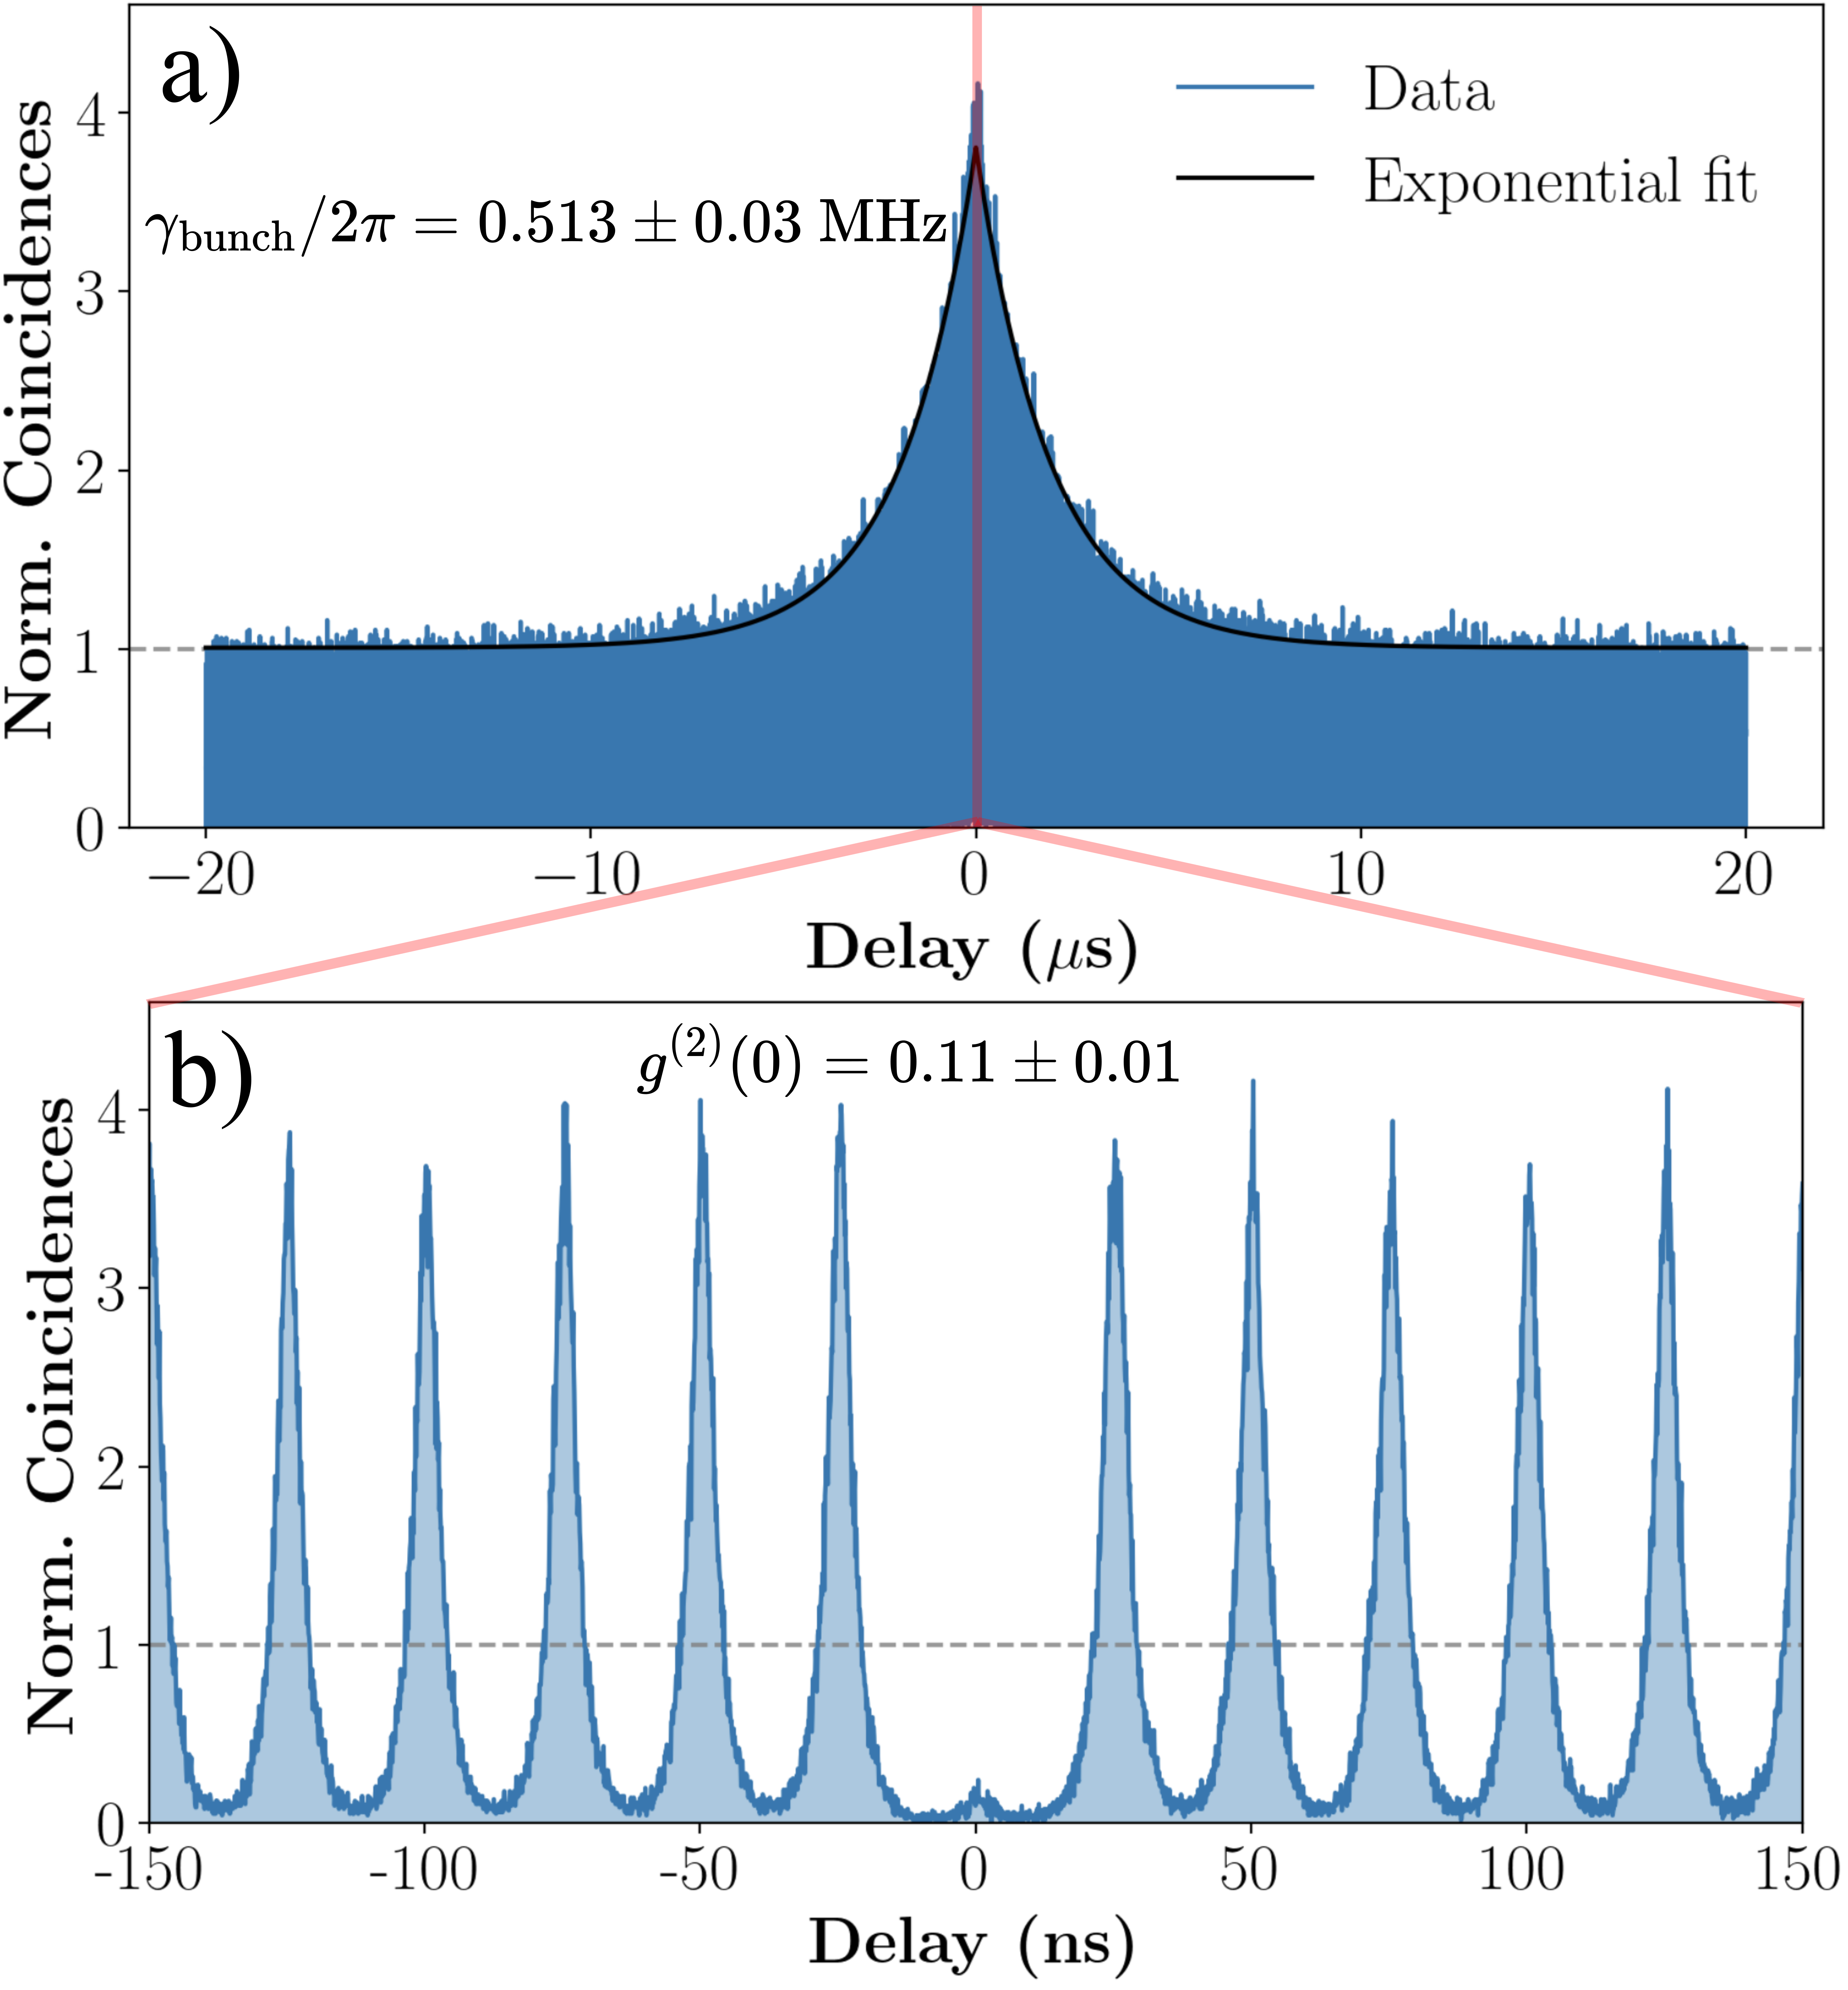
\includegraphics[width=0.8\linewidth]{Figures/pulsedg2.png}
    \caption{Graphs of $g^{(2)}(\tau)$ normalised to long delays under pulsed excitation conditions at 40 MHz and $1.2P^{\text{p}}_{\text{Sat}}$, Fig.~\ref{fig:laser-char}c. Panel (a) shows the data (blue lines) to long time delays. The decay envelope is fitted with an exponential to extract the bunching rate, found to be $\gamma_{\text{bunch}}/2\pi=0.513\pm0.003 \ \text{MHz}$. The bottom panel (b) is the central part of the $g^{(2)}(\tau)$ data, and $g^{(2)}(0)$ is calculated to be $g^{(2)}(0) = 0.11 \pm 0.01$.} 
    \label{fig:pulsedg2}
\end{figure}

Fig.~\ref{fig:pulsedg2}a shows the $g^{(2)}(\tau)$ data of the 710 nm defect under pulsed excitation at 40 MHz and $1.2P^{\text{p}}_{\text{Sat}}$. Prominent bunching is evident, with peak heights about four times those at long delays. To analyse this, the envelope was fitted with a symmetric exponentially decaying function (black line), yielding a bunching rate of $\gamma_{\text{bunch}}/2\pi=0.513\pm0.003$ MHz. This decay suggests the involvement of a metastable dark state consistent with a three-level system~\cite{Boll2020}. Notably, the spontaneous decay rate $\gamma$ is about a thousand times faster than $\gamma_{\text{bunch}}$, so the radiative lifetime still governs the emission timescale.


Fig.~\ref{fig:pulsedg2}b presents the central peak of the $g^{(2)}(\tau)$ data. The grey dashed line shows the height of the peaks at long time delays. To calculate the $g^{(2)}(0)$, the area of the central peak at zero time delay is divided by the average area of peaks at long time delay. The area of each peak that is integrated is an important factor when calculating the $g^{(2)}(0)$. In order to determine the appropriate window size, $g^{(2)}(0)$ is calculated for integration windows ranging from 1 to 200 points on either side of the peak maximum, as shown in Fig.~\ref{fig:g2window}a. The final window size is selected manually by identifying a region where the gradient of $g^{(2)}(0)$ with respect to the window size is small, so that a small change in window size does not massively affect the $g^{(2)}(0)$, but not 0. The window integration size is taken as 50 (red dot Fig.~\ref{fig:g2window}). The data lying between outside of the window, between adjacent peaks, is split into three sections (green and red section Fig.~\ref{fig:g2window}b), and the middle section is taken as the background noise of the measurement (red lines Fig.~\ref{fig:g2window})b. The average background value is subtracted from all other data points, or zero is used where this subtraction would result in negative values.The area under the central peak, and the average area under the peaks at long time delays is calculated, yielding $g^{(2)}(0) = 0.11 \pm 0.01$. The error is calculated using the standard deviation of the peak areas at long time delays, and by assuming Poissonian statistics for the central peak. From the pulsed $g^{(2)}(0)$, the purity is found to be $P=0.89$, which is comparable to other hBN defects reported at room temperature \cite{Zeng2022, Grosso2017, Vogl2017}.


\begin{figure}[h!]
    \centering
    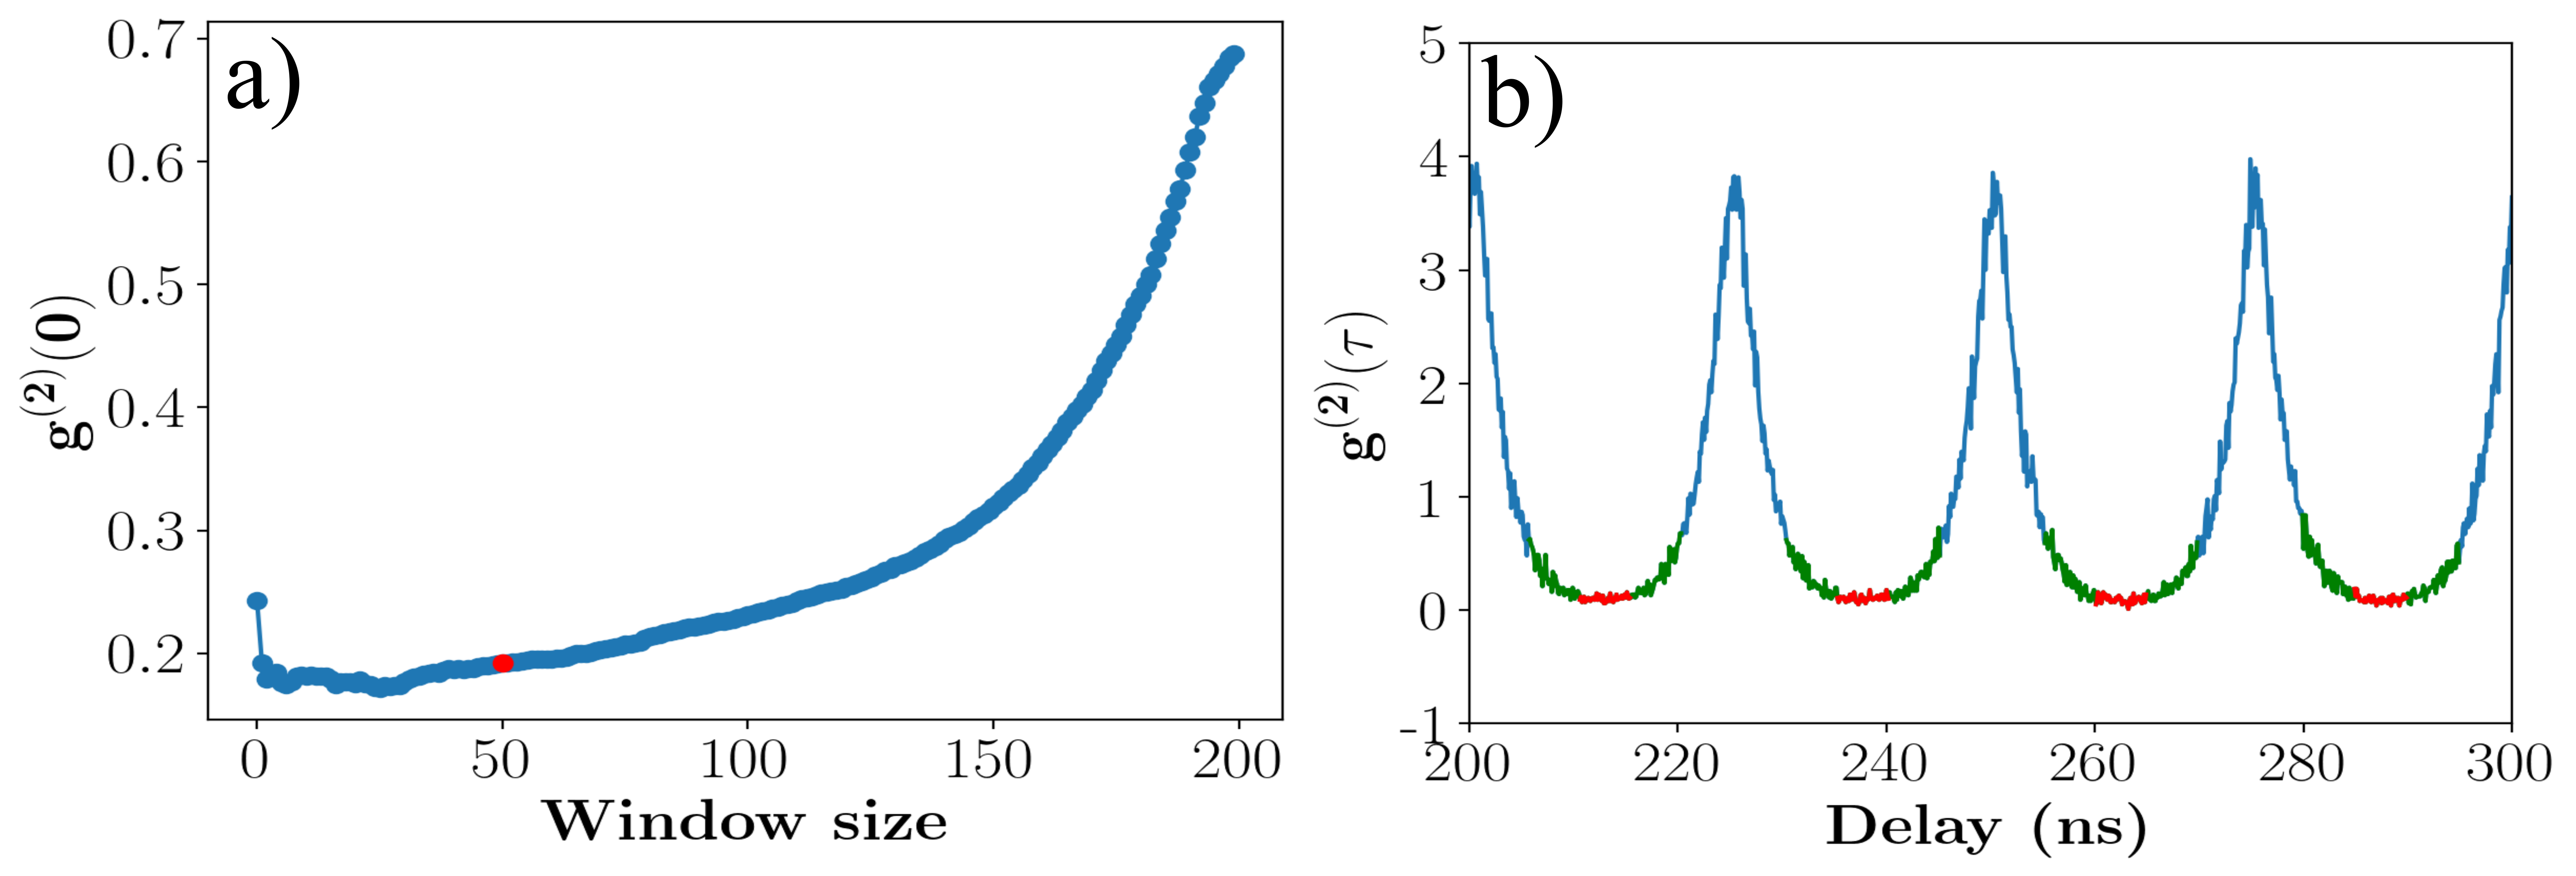
\includegraphics[width=1\linewidth]{Figures/g2window.png}
    \caption{a) Calculated $g^{(2)}(0)$ for integration window sizes between 1 and 200 points either side of each paks maximum before background removal. b) Example of thearea outside of each window being split into 3, with the middle part (red) being taken as the background noise of the measurement}
    \label{fig:g2window}
\end{figure}

Fig.~\ref{fig:cwg2} presents the normalised power-dependent $g^{(2)}(\tau)$ under CW excitation. There is a clear increase in photon bunching with excitation power, which can be understood by considering that higher excitation rates increase the likelihood of the emitter being promoted into the metastable dark state discussed in the pulsed $g^{(2)}(\tau)$ analysis. This leads to longer periods during which the emitter is non-emissive, thereby increasing the correlations observed in the bunching tail. The coefficients of the the bi-exponential fits, Eqn.~\ref{eqn:bi-decay-g2}, (black lines) are displayed in table~\ref{tab:g2coeff}. The increase in magnitude of the coefficients implies larger bunching. 

\begin{figure}[h!]
    \centering
    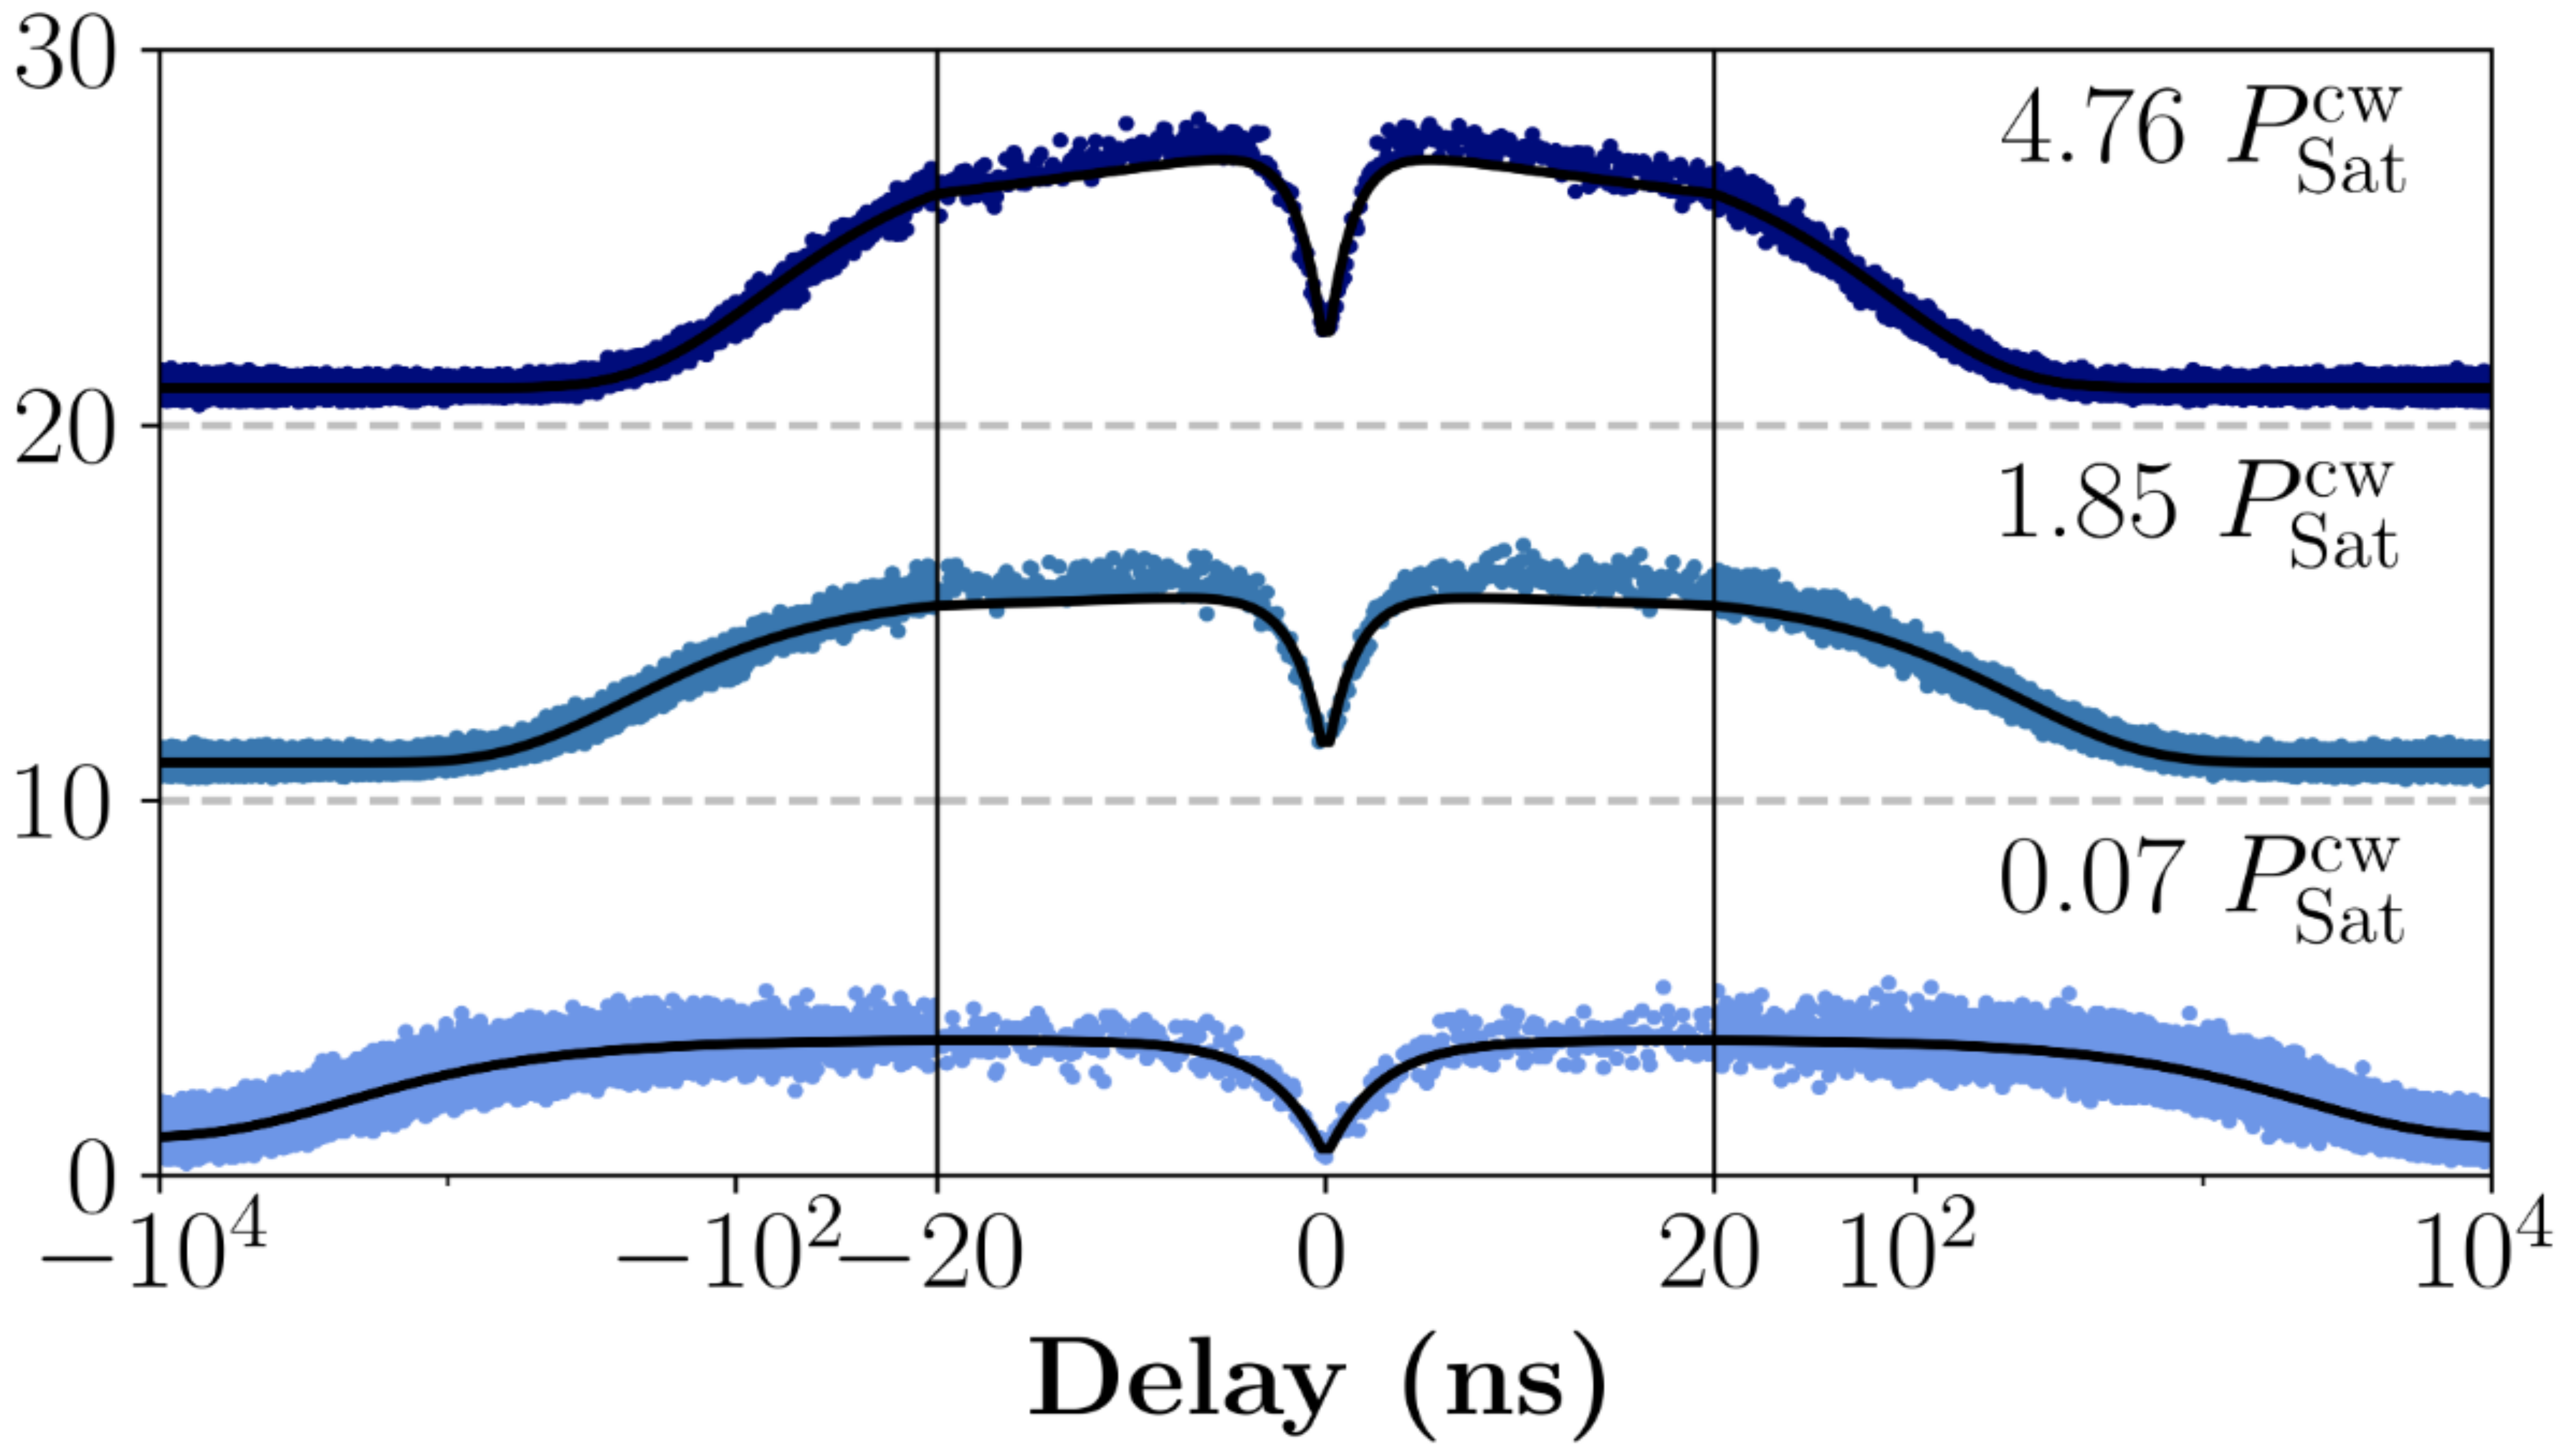
\includegraphics[width=0.9\linewidth]{Figures/CWg2.png}
    \caption{$g^{(2)}(\tau)$ under CW excitation for various powers relative to the saturation power of the emitter, $P_{\text{Sat}}^{\text{cw}}$}
    \label{fig:cwg2}
\end{figure}

\begin{table}[h!]
\centering
\begin{tabular}{|c|c|c|c|c|}
\hline
\textbf{Power ($P^{\text{cw}}_{\text{Sat}}$)} & $A$ & $B$ & $C$ & $g^{(2)}(0)$ \\
\hline
0.07 &     24.73$\pm$0.02     &   -77.27$\pm$1.40  & 64.81$\pm$0.08   & 0.50$\pm$0.06 \\
\hline
1.85 &      78.47$\pm$0.02      &    -360.0$\pm$4.9  & 358.0$\pm$0.6& 0.97$\pm$0.06 \\
\hline
4.76 &      89.11$\pm$0.02       &    -528.0$\pm$6.7   & 587.7$\pm$1.2   & 1.67$\pm$0.08 \\
\hline
\end{tabular}
\caption{Coefficients resulting from applying a bi-exponential fit to the $g^{(2)}(\tau)$ data for each excitation power.}
\label{tab:g2coeff}
\end{table}

The elevated $g^{(2)}(0)$ values can be attributed to the limited temporal resolution of the detectors, which is comparable to the anti-bunching timescale $\tau_0$ near zero delay, table~\ref{tab:g2time}. In principle, deconvolution of the data with the IRF of the APDs (see Fig.~\ref{fig:apd-characterisation}) would be required to accurately extract $g^{(2)}(0)$. However, this was deemed unnecessary here, as the pulsed excitation measurements (Fig.~\ref{fig:g2window}a) provides independent confirmation of single-photon emission.

\begin{table}[h!]
\centering
\begin{tabular}{|c|c|c|c|c|}
\hline
\textbf{Power ($P^{\text{cw}}_{\text{Sat}}$)} & $\mathbf{\tau_0 \ (ns)}$ & $\gamma_0/2\pi$ (GHz)& $\mathbf{\tau_1 \ (ns)}$ & $\gamma_1/2\pi$ (MHz) \\
\hline
0.07 &     $2.78\pm0.10$        &  0.36$\pm$0.01  &  $2279\pm6$ & 0.438$\pm$0.001\\
\hline
1.85 &      $1.49\pm0.04$       &   0.67$\pm$0.02  &  $235\pm1$  & 4.24$\pm$0.02\\
\hline
4.76 &      $1.31\pm0.03$       &   0.76$\pm$0.02  &  $82\pm1$   &  12.2$\pm$0.2\\
\hline
\end{tabular}
\caption{Decay times and rated for CW driven $g^{(2)}(\tau)$.}
\label{tab:g2time}
\end{table}

The effect of pump power on the emitter’s dynamics is evident from changes in both antibunching and bunching timescales, with higher powers exhibiting larger blinking effects. At the lowest power, the antibunching rate ($\gamma_0$) is similar to that of the emitters lifetime. However, as the power increases, so does $\gamma_0$. Similar behaviour is exhibited by the bunching rate ($\gamma_0$), where it is initially comparable to $\gamma_{\text{bunch}}$ under pulsed excitation. The increase in these rates is due to faster cycling between the ground and excited states, and consequently shorter characteristic decay times. 

\subsubsection{Indistinguishability}

The indistinguishability of the 710 nm defect is measured using a Michelson interferometer along with the lifetime results from section~\ref{spec-lt}. The Michelson interferometer is used to measure the total dephasing rate of the emitter under different excitation powers and filtering conditions.

\begin{figure}[h!]
        \centering
        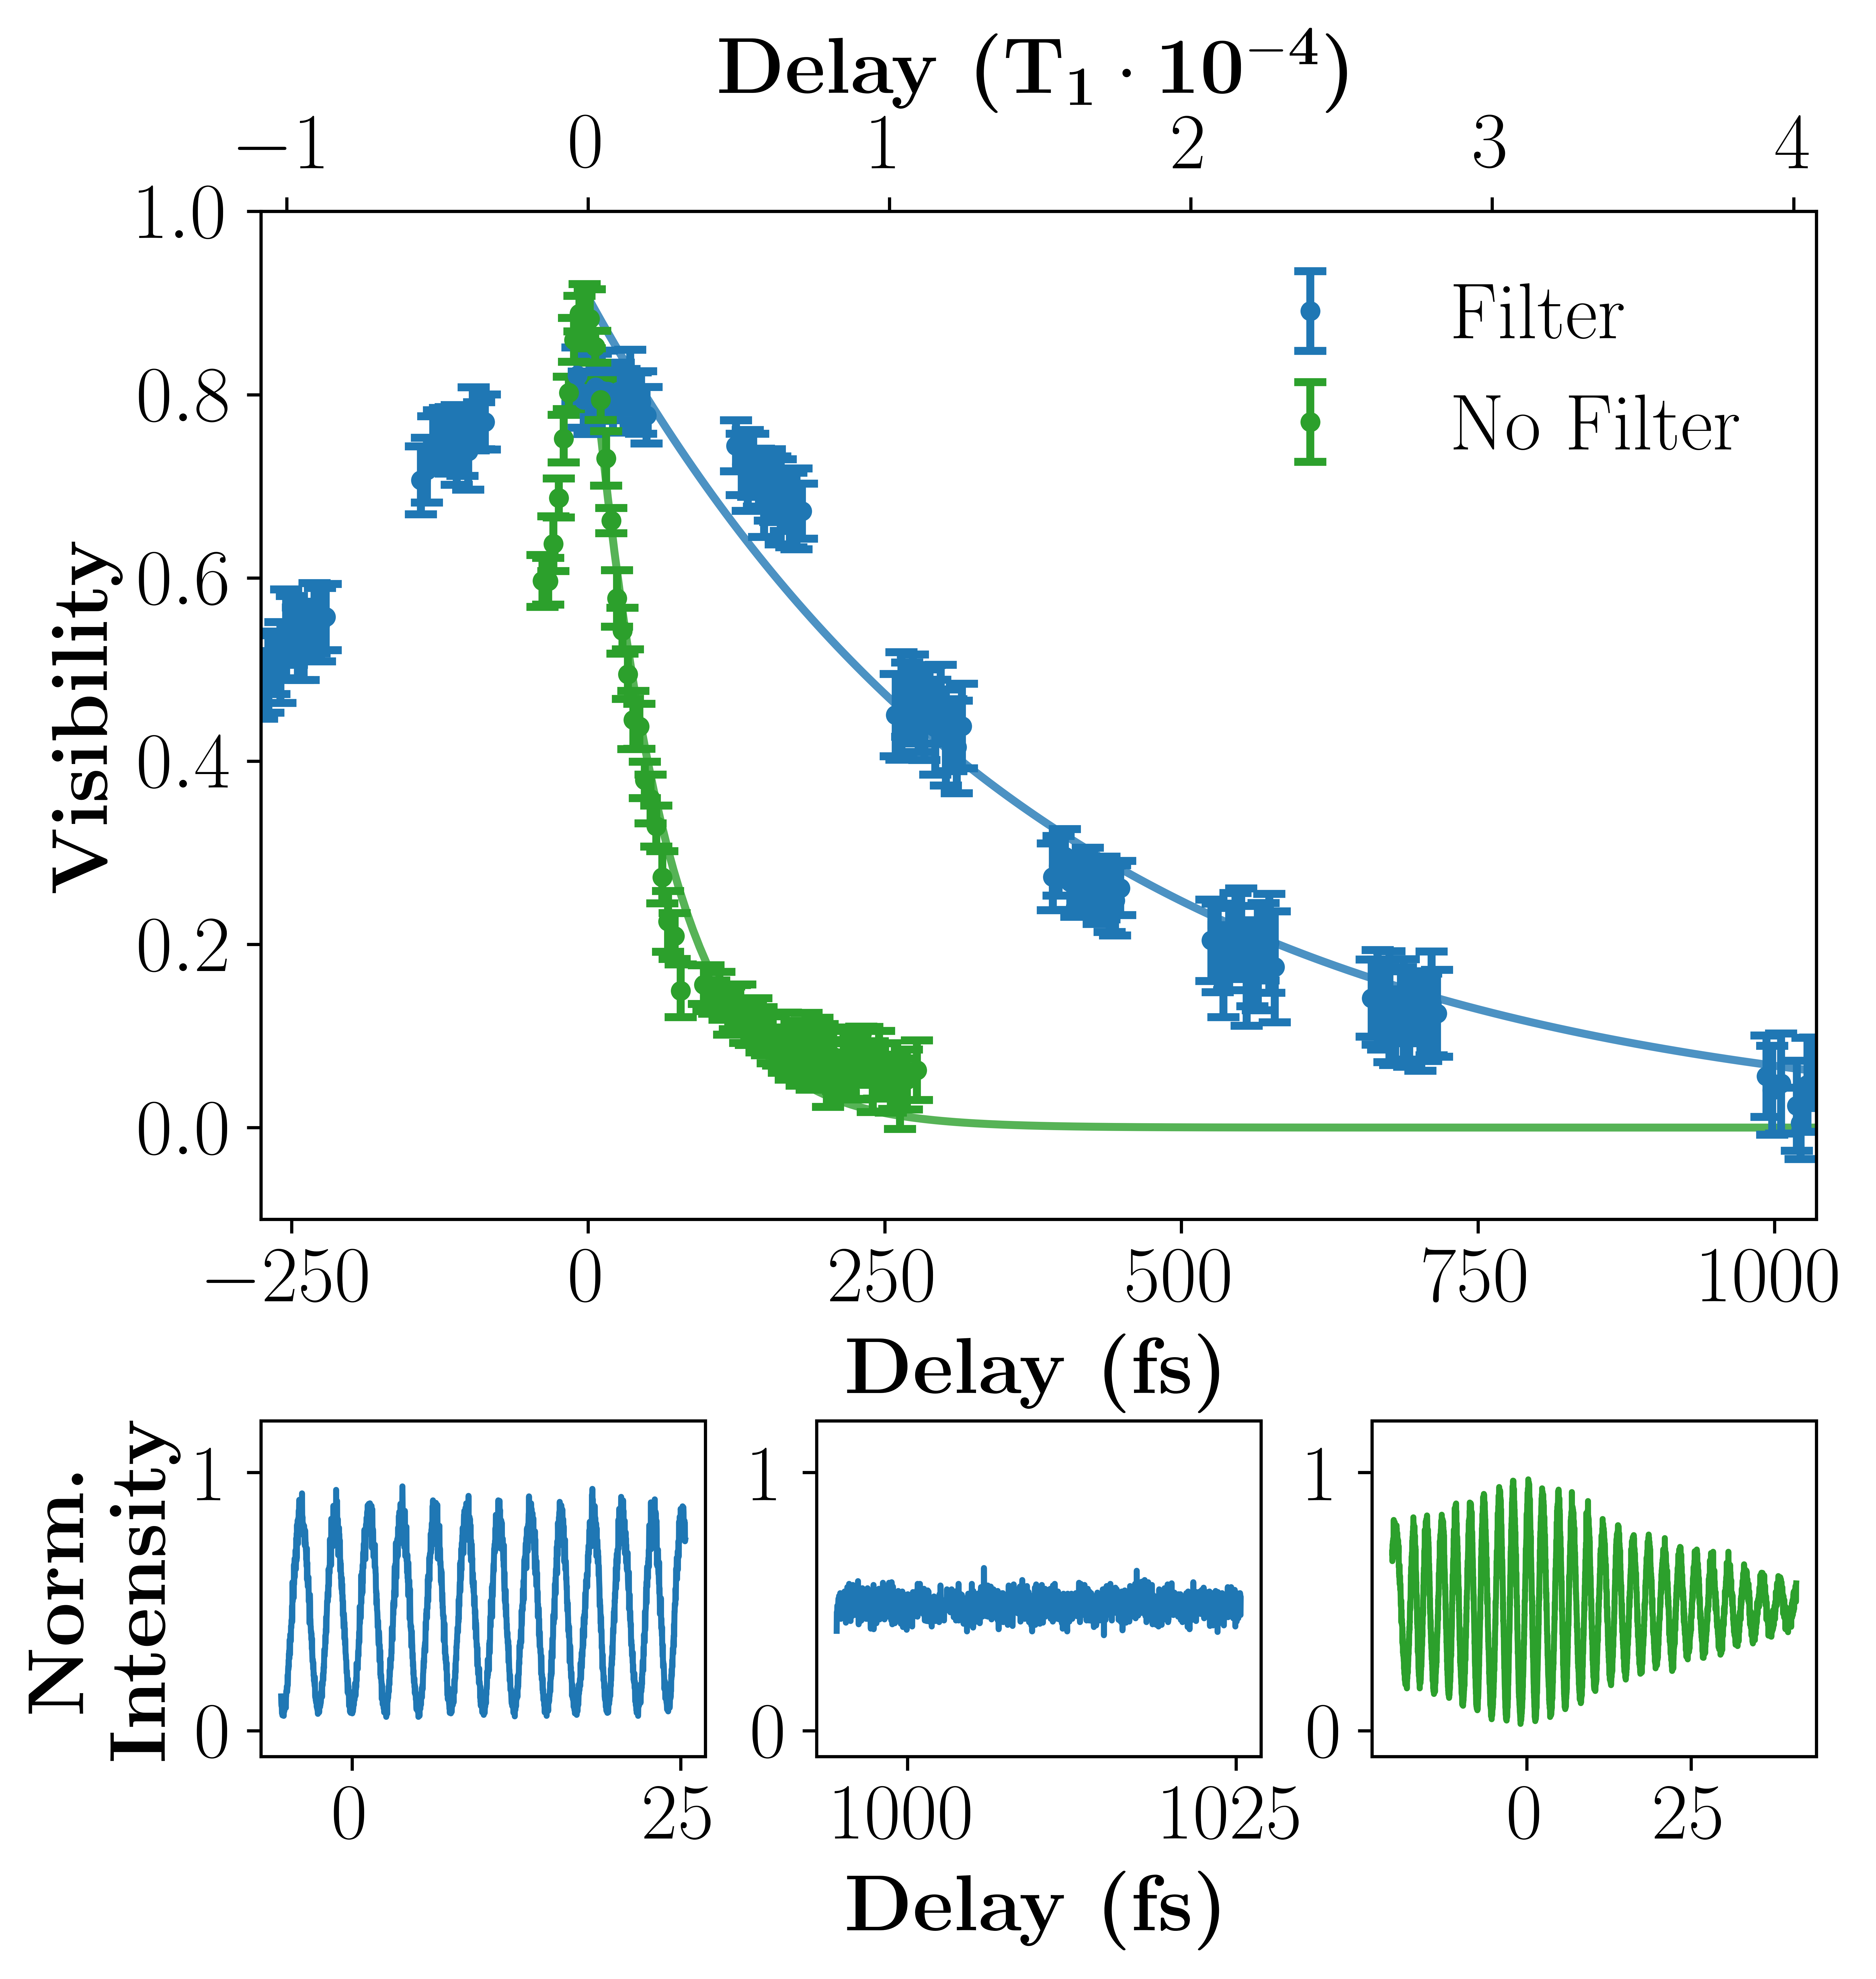
\includegraphics[width=0.8\linewidth]{Figures/FilterVis.png}
        \caption{Visibility vs. delay for filtered ZPL (black) and unfiltered ZPL+PSB (green). Interference patterns at various delays can be seen in the bottom panels.}
        \label{fig:filter-vis}
\end{figure}

Fig.~\ref{fig:filter-vis} presents the results of the visibility measurements under different spectral filtering conditions. The defect was driven at 1.85$P_{\text{Sat}}^{\text{cw}}$ using the CW setting. The blue data points correspond to photons collected from the filtered ZPL (grey area Fig.~\ref{fig:spectra}a) where the contributions from the PSB are excluded. The data points represent the visibility of an individual interference oscillation. The green data points represent measurements taken with a partially filtered spectrum, including both ZPL and PSB photons, as indicated by the green dashed line in Fig.\ref{fig:spectra}a. The lower panels display the corresponding intensity oscillations as a function of time delay, which follow the decay behaviour described by Eqn.~\ref{eqn:int-decay}. Notably, the oscillations in the filtered ZPL case decay significantly more slowly than those of the partially filtered spectrum, indicating longer coherence. For each delay position, the visibility was calculated by taking the mean and standard deviation of 20 data points around the interference peak. Standard error propagation formulas were then applied to determine the uncertainty in the extracted visibility. These visibility values were subsequently fitted using an exponential decay model, as described by Eqn.~\ref{eqn:vis-decay}. 

The filtered ZPL exhibits a total dephasing rate of $\Gamma/2\pi = 5.24 \pm 0.16$~THz, corresponding to a coherence time of $T_2 = \frac{2}{\Gamma/2\pi} = 0.382 \pm 0.011$~ps. From this, the pure dephasing rate can be measured as $\gamma^*/2\pi = \frac{\Gamma/2\pi - \gamma/2\pi}{2} \approx \frac{\Gamma/2\pi}{2} = 2.62 \pm 0.08$~THz. The resulting photon indistinguishability is $I = \frac{\gamma}{\Gamma} \approx 0.0075\%$. In contrast, the partially filtered ZPL, where both PSB and ZPL photons contribute, shows significantly faster decoherence. The visibility decay yields a total dephasing rate of $\Gamma/2\pi = 29.4 \pm 0.2$~THz, corresponding to a much shorter coherence time of $T_2 = 0.0680 \pm 0.0005$~ps and a pure dephasing rate of $\gamma^*/2\pi = 14.7 \pm 0.1$~THz. The inclusion of incoherent PSB photons greatly accelerates the dephasing and reduces the indistinguishability to $I = 0.0013\%$. The fact that the visibility peaks at 80\% is an indicator that the spatial alignment of the interferometer is not perfect. These results clearly demonstrate that spectral filtering of the ZPL significantly reduces the dephasing rate. Further improvements to the indistinguishability could be achieved by combining spectral filtering with temporal filtering, as demonstrated in Ref.~\cite{Fournier2023}.

\begin{figure}[h!]
        \centering
            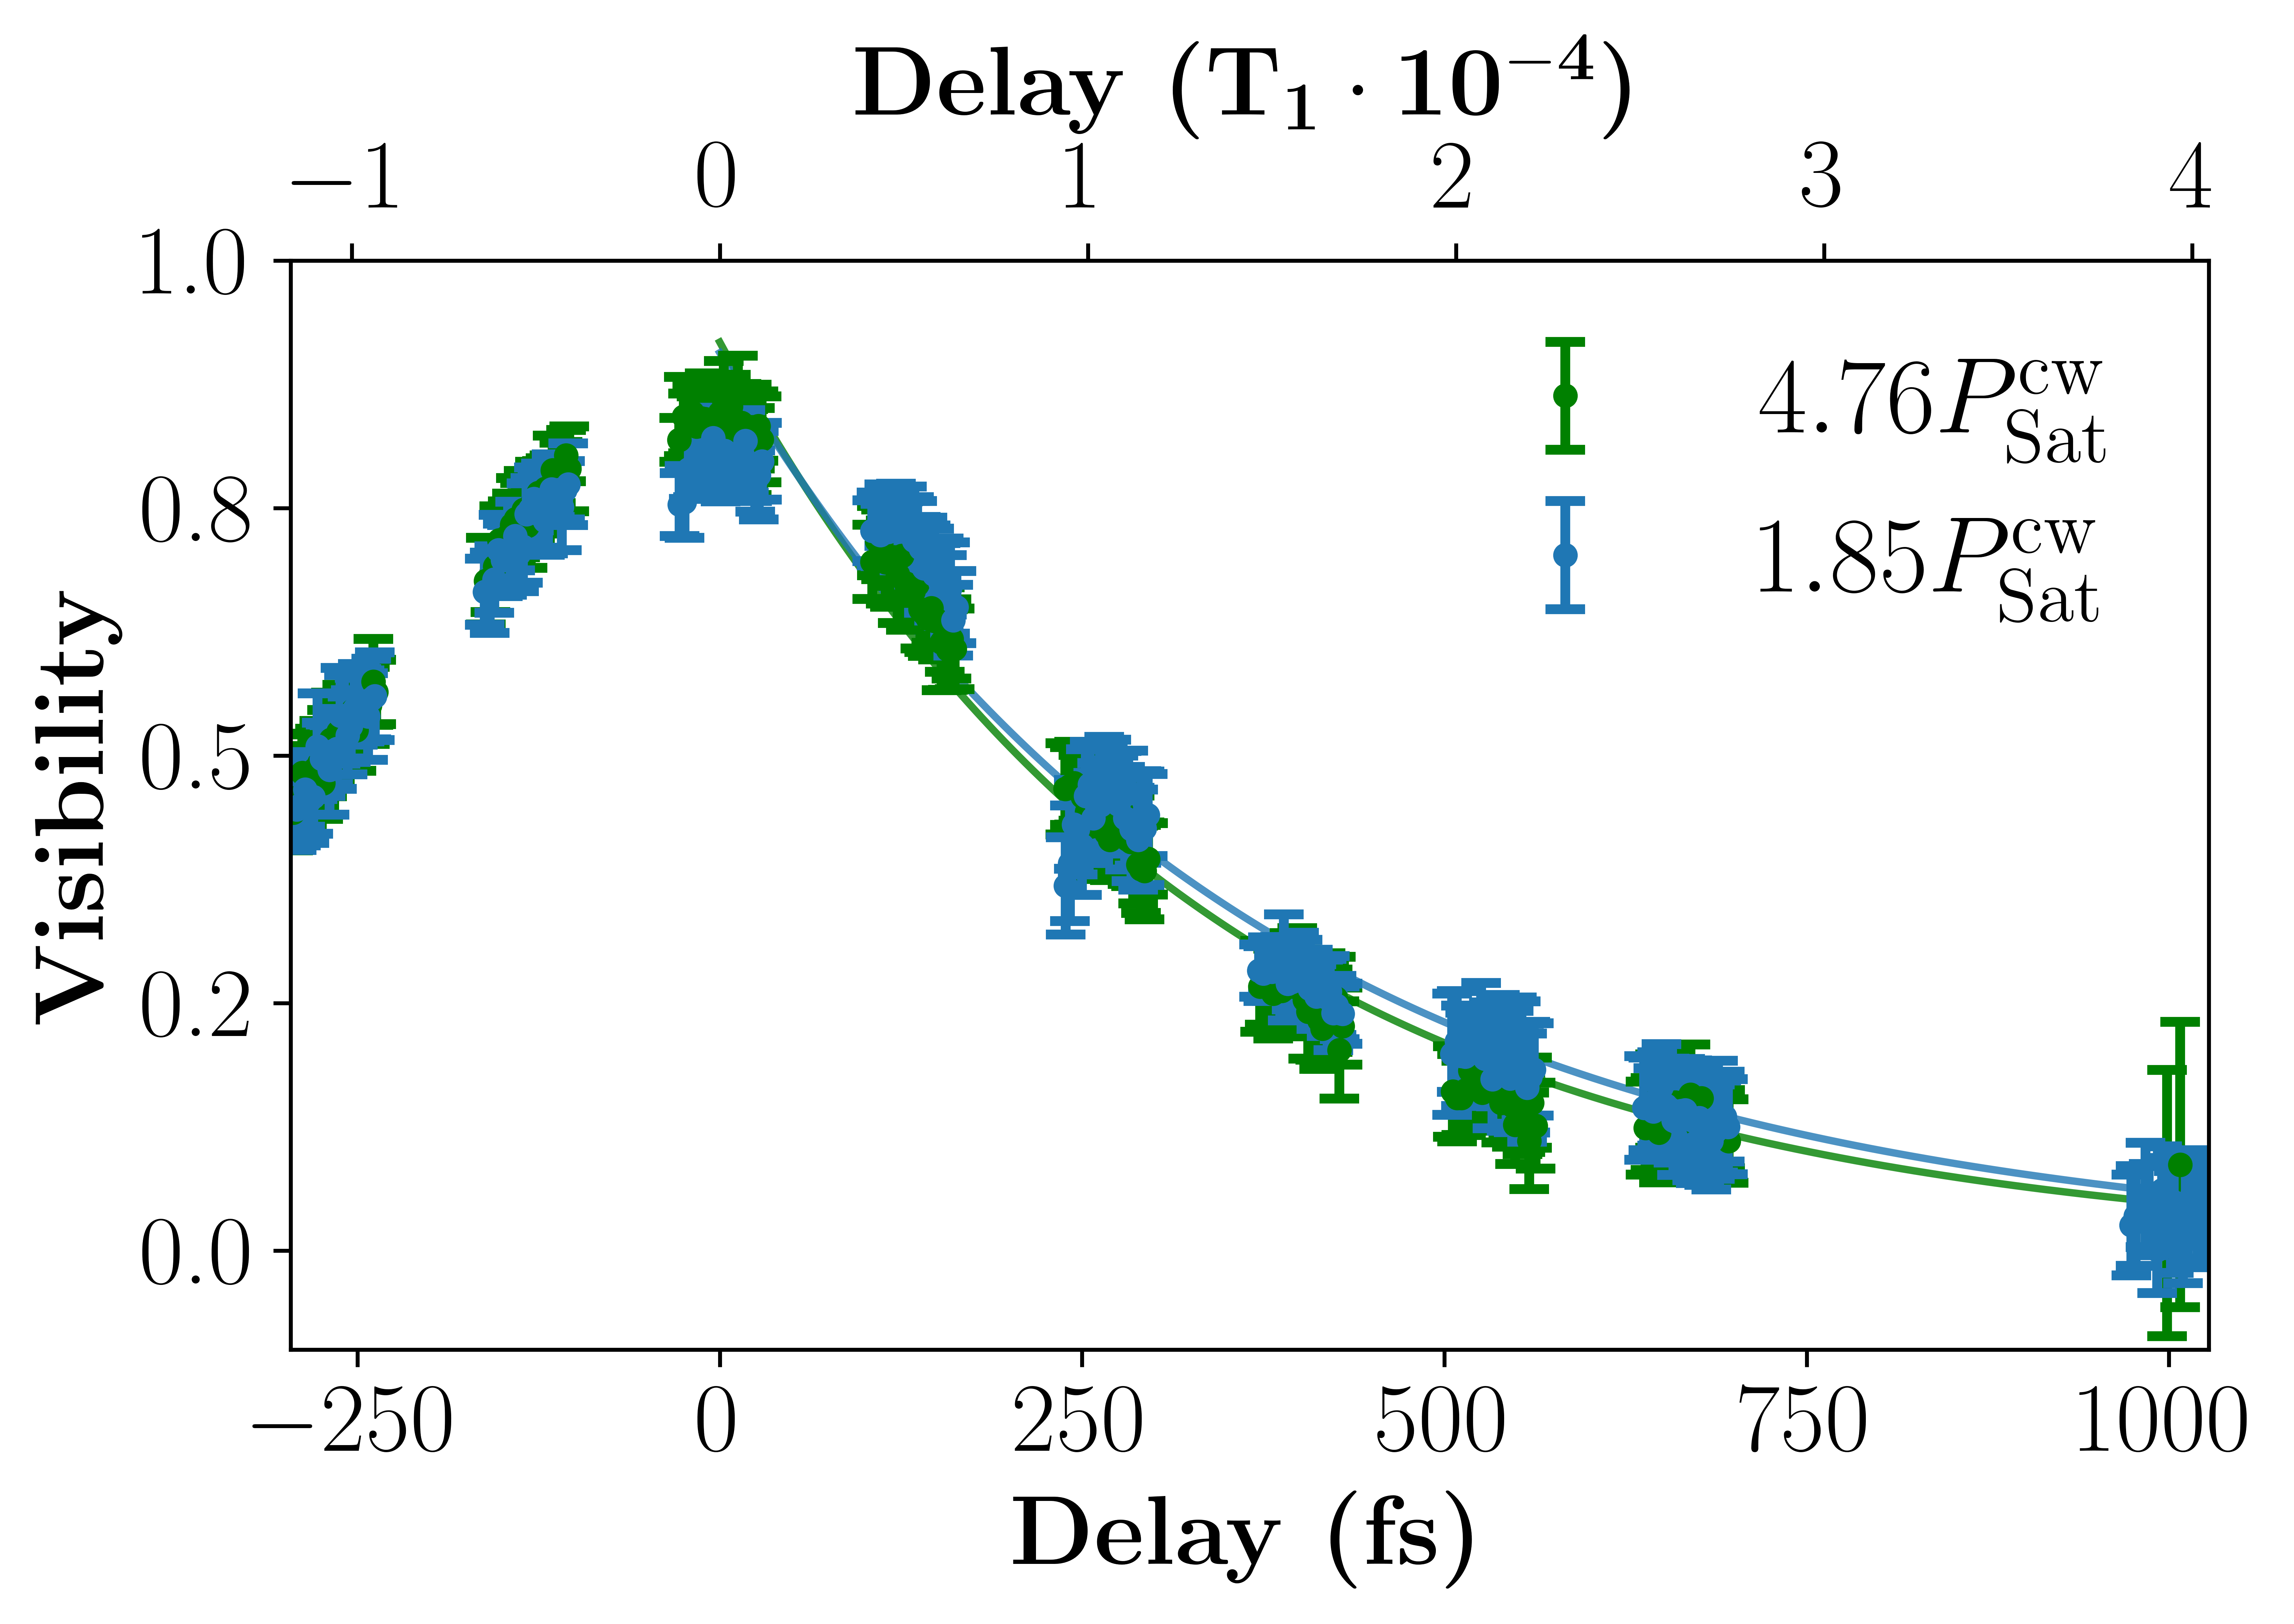
\includegraphics[width=0.8\linewidth]{Figures/PowerVis.png}
        \caption{Power-dependent visibility measurements, demonstrating the effect of excitation power on coherence properties.}
        \label{fig:power-vis}
\end{figure}


The effect of excitation power on indistinguishability was investigated by measuring visibility decay at two pump powers, $4.76P_{\text{Sat}}^{\text{cw}}$ and $1.85P_{\text{Sat}}^{\text{cw}}$, shown in Fig.~\ref{fig:power-vis}. The results indicate that excitation power does not significantly affect indistinguishability: the extracted total dephasing rates differed by less than 8\%, comparable to the measurement uncertainty. This suggests excitation-induced dephasing does not impact photon coherence within the examined power range and validates the choice of power for the previous measurements.

The discrepancy between the measured total dephasing rate, $\Gamma/2\pi = 5.25 \pm 0.16$~THz, and the FWHM of 1.2~THz (a spectral width difference of ~5 nm) is attributed to the non-exponential, Gaussian-like visibility decay. According to the Wigner-Khinchin theorem, the emitter spectrum is the Fourier transform of its first-order coherence function $g^{(1)}(\tau)$. While an unfiltered Lorentzian spectrum yields an exponential decay, the bandpass filters truncate the ZPL shoulders, reshaping the emission and producing a Gaussian-like decay. To confirm this, the Fourier transform of the filtered ZPL spectrum was computed, as shown in Fig.~\ref{fig:FT-spec}, where the transformed coherence function closely matches the measured visibility decay.

Excellent agreement between the experimental data and the Fourier-transformed spectrum confirms that spectral filtering significantly alters the temporal coherence function and is responsible for the observed Gaussian decay envelope.

\begin{figure}[h]
    \centering
    \includegraphics[width=1\linewidth]{Figures/FTSpec.png}
    \caption{(Left) Filtered ZPL emission spectrum. (Right) Measured visibility as a function of optical delay (blue) compared to the Fourier transform of the filtered ZPL spectrum (orange). The agreement supports the interpretation that spectral filtering modifies the temporal coherence and gives rise to a Gaussian-shaped visibility decay.}
    \label{fig:FT-spec}
\end{figure}

While one could argue that the Michelson interferometry measurement is unnecessary due to the Fourier transform relationship between the emission spectrum and the temporal coherence function, the direct measurement of visibility decay for hBN emission at room temperature represents a novel and valuable contribution. Unlike coherence times sourced from spectral measurements, which require post-processing steps such as background subtraction and spectral centring, interferometric measurements provide a more direct and reliable measyre of the first-order coherence. Although only a single emitter was fully characterised in this work, many hBN flakes exhibited emission with similar characteristics to the emitter investigated as presented in Figs.~\ref{fig:spectra},\ref{fig:lifetimes} .The results in the preceding sections highlight the significant potential of hBN defect emission for room-temperature quantum applications that do not require photon indistinguishability, such as QKD. However, as expected, strong electron–phonon coupling at room temperature introduces substantial dephasing, making these emitters unsuitable for applications that rely on photon self-interference, such as distributed entanglement for communication or computation. To improve the performance of hBN-based single-photon sources at room temperature, it is essential to integrate them into optical cavities. Such cavity structures can enhance the spontaneous emission rate via the Purcell effect, thereby increasing the brightness and overall utility of the source \cite{Nonahal2023}.

\subsection{Future experiments}

Although stand-alone hBN defects exhibit promising properties for quantum photonic technologies, their performance can be further enhanced through cavity quantum electrodynamic effects \cite{Kimble1998}. Placing an emitter inside an optical cavity introduces an additional decay channel alongside the intrinsic radiative ($\gamma_{\text{rad}}$) and non-radiative ($\gamma_{\text{nrad}}$) decay rates, resulting in a total emission rate $\gamma' = \gamma_{\text{rad}} + \gamma_{\text{nrad}} + \gamma_{\text{cav}}$ \cite{Auffeves2010}. The interaction between an emitter and a cavity mode is described by a Jaynes–Cummings type Hamiltonian with a coupling strength $g \propto 1/\sqrt{V}$, where $V$ is the cavity mode volume. $V$ quantifies the spatial extent of the confined electromagnetic field. The cavity emits energy at a rate determined by its linewidth $\kappa$, and in the weak coupling regime ($2g \ll \kappa$), coherent energy exchange is negligible compared to losses, and the system behaves effectively as an emitter with an enhanced radiative decay rate. Here, the radiative decay into the cavity mode is given by $\gamma_{\text{cav}} = \frac{4g^2}{\kappa + \Gamma}$, with $\Gamma$ the emitter's linewidth, and the cavity quality factor is defined as $Q = \omega_c/\kappa$.

In the ideal case $\Gamma \ll \kappa$, the Purcell factor $F_P \propto Q/V$ describes the enhancement of the emitter’s radiative decay rate. Assuming the emitter is correctly positioned and spectrally matched to the cavity mode, the total decay rate becomes $\gamma' = \gamma + F_P \gamma_{\text{rad}}$. This captures how the cavity modifies the photonic environment to increase radiative emission. Purcell enhancement has been demonstrated in systems such as semiconductor quantum dots embedded in micropillar cavities \cite{Engel2023} and organic dye molecules coupled to plasmonic nanoantennas \cite{Zhao2020}.

Future experiments should investigate coupling hBN emission into open optical cavity modes to exploit the Purcell effect further. An open Fabry–Pérot cavity, supporting resonant modes defined by $L = n\lambda/2$, where $L$ is the cavity length, offers one practical approach. For a plano–plano cavity, the mode volume is approximated by $V = L \times A$, so reducing the mirror separation can decrease $V$ while maintaining a stable $Q$. Such cavity-enhanced systems could not only improve the brightness of single-photon sources but also increase photon indistinguishability by acting as narrow spectral filters that enhance resonant emission and suppress off-resonant components.


